\documentclass[a4paper]{article}

\usepackage{amsmath,amsthm,amssymb}
\usepackage{tikz}
\usetikzlibrary{arrows}
\usetikzlibrary{external}
\tikzexternalize[prefix=figures/]

\tikzset{
every node/.style={circle, draw, inner sep=2pt},
every label/.style={rectangle, draw=none}
}

\begin{document}

%%%%%%%%%%%%%%%%%%%%%%%%%%%%%%%%%%%%%%%%%%%%%%%%%%
\verb|minspan|

\tikzsetnextfilename{minspan}
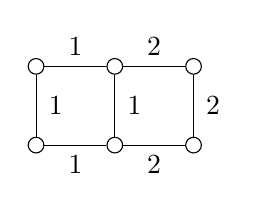
\begin{tikzpicture}
\node (1) at (0,0) {};
\node (2) at (1,0) {};
\node (3) at (2,0) {};
\node (4) at (0,1) {};
\node (5) at (1,1) {};
\node (6) at (2,1) {};

\draw (1) --node[midway,below,draw=none] {$1$} (2);
\draw (4) --node[midway,above,draw=none] {$1$} (5);
\draw (1) --node[midway,right,draw=none] {$1$} (4);
\draw (2) --node[midway,right,draw=none] {$1$} (5);
\draw (2) --node[midway,below,draw=none] {$2$} (3);
\draw (5) --node[midway,above,draw=none] {$2$} (6);
\draw (3) --node[midway,right,draw=none] {$2$} (6);
\end{tikzpicture}

\end{document}


%%% compile by pdflatex --shell-escape filename.tex
%%% then run ./pdf2png.sh *.pdf in figures/
